\documentclass{bioinfo}
\copyrightyear{2017}
\pubyear{2017}

\begin{document}
\firstpage{1}

\title[WhiH Motif discovery]{Motif discovery and its analysis for binding sites of WhiH (White H) transcription factor in Streptomyces}
\author[Gladchuk \textit{et~al}]{Sergii Gladchuk\,\footnote{to whom correspondence should be addressed}, Klas Fl{\"a}rdh\, and Bj{\"o}rn Canb{\"a}ck\,}

\address{Department of Biology, Box 118, 221 00, Lund University, Sweden}

\history{Received on XXXXX; revised on XXXXX; accepted on XXXXX}

\editor{Associate Editor: XXXXXXX}

\maketitle

\begin{abstract}

\section{Motivation:}
The aim of the developed procedure was to discover and analyze sequence motifs based on results of ChIP-seq experiments with MEME suit that may constitute binding sites for the WhiH protein. The initial procedure described in MEME manual required to much manual conversions and input data modifications in order to get appropriate input for MEME-ChIP program. Also further motif correlation with expression data has to be confirmed.

\section{Results:}
Set of steps and scripts where developed to facilitate whole motif discovery procedure and ChIP-seq/motifs correlation with expression data. The final statistical analysis confirmed success of ChIP-seq experiment and produced list of motif-relevant significantly over-/under-expressed genes, which can  illuminate the mechanism of transcriptional regulation.

\section{Availability:}
Detailed description of full analysis together with all the results can be found on public repository (under results folder, notebook.html): \href{https://github.com/sergiigladchuk/WhiH\_motiff}{https://github.com/sergiigladchuk/WhiH\_motiff}

\section{Contact:} \href{se1522gl-s@student.lu.se}{se1522gl-s@student.lu.se}
\end{abstract}

\section{Introduction}

WhiH is a transcriptional regulator of the GntR family that controls late stages of sporulation and cell division in Streptomyces. Chromatin Immuno Precipitation followed by next generation sequencing (ChIP-seq) experiment has been conducted to identify regions of DNA that are bound by WhiH during sporulation of the model organism Streptomyces venezuelae. Identifying a main motif in a large fraction of the peaks by motif analysis can confirm successful experiment and also identify the DNA-binding motifs of other proteins that bind in complex or in conjunction with the ChIPed protein, illuminating the mechanisms of transcriptional regulation (\citealp{MEME}).\\
In addition, microarray-based transcriptomic analyses have also been performed to monitor patterns of gene expression in wild type and whiH mutant strains during growth and sporulation.\\
Initial analysis of the data showed that WhiH has very complex regulon structure and motif discovery together with expression data correlation can better identify genes, which are under direct WhiH control.

\begin{methods}
\section{Methods}


{\bf Chromatin immunoprecipitation, library construction, sequencing, and ChIP-seq data analysis} were performed by The Genome Analysis Centre (TGAC), Norwich Research Park Norwich, United Kingdom, as described in \citealp{Bush2013}.\\
{\bf Motif discovery} based on ChIP-seq peaks data provided. Two lists (all significant peaks  and top 36 peaks), which correspond to genomic coordinates in {\it S. venezuelae} genome (Gen-Bank accession number NC\_018750, \citealp{Genome}), were separately used to extract 500-nucleotide-long ranges with python script {\it seq\_extractor}. These ranges where fed to MEME-ChIP program (\citealp{MEME}). Numerous settings (different level Markov Models for background, palindromic only, discriminative mode) in different combinations were applied to make motiff more specific and show better back-check results based on FIMO program from MEME suit, which match given motif to the genome. Only 4 best motifs were selected for further statistical analysis:

\begin{itemize}
\item 'Best TOP non-palindromic discriminative motif’ discovered with MEME-ChIP (settings: discriminative mode against 500 random ranges with 0-model background, non-palindromic, based on TOP ChIP-seq regions)
\item 'TOP palindromic motif' - discovered with MEME (settings: background Markov model order 0 with palindrome only, based on TOP ChIP-seq regions)
\item 'Best ALL-Peaks back-check discriminative motif' discovered with MEME-ChIP (settings: 10000 random ranges with 0-model background, non-palindromic, based on ALL ChIP-seq regions)
\item 'Best e-value from ALL peaks' - discovered with MEME (settings: background Markov model order 0, non-palindromic, based on ALL ChIP-seq regions)\\
\end{itemize}

{\bf Statistical analysis} for expression dependency of genes in close proximity to discovered motifs was done in R. For each selected motif list of positions from FIMO program was used to identify nearby genes on both DNA strands with developed python program {\it affy\_log\_creator}. This script takes 3 inputs: transcriptomics data file, annotation file of all genes for {\it S. venezuelae} and list of positions. It converts transcriptomics into AffyLog levels for each gene, and marks genes winch have motif position in region - 300 away from the start codon and +50 after start codon.\\
Same {\it affy\_log\_creator} program was used to produce list of all genes with expression level and marked related genes from PREDetector program (\citealp{Predetector}) and initial ChIP-seq peak positions.\\
Produced gene lists with AffyLogs and marked genes were used in actual statistical analysis in R. Procedure of the analysis:

\begin{enumerate}
\item whole list was processed 7 times (from 8h to 20h separately)
\item based on each time AffyLogs values gene list was split into two lists - over- and under- expressed genes (AffyLog - (-) indicates a decrease in expression of the gene in a whiH mutant compared to the wild-type; (+) indicates an increase in expression of the gene in a whiH mutant compared to the wild-type)
\item these sub-lists with two categories of genes (‘special’ genes marked due to closeness to Motif or ChIP-seq peak and ‘all other non-related’ genes) were fed to one-sided Mann‐Whitney non-parametric independent samples test to find significant difference in variation of expression data for two categories. This non-parametric test was chosen because data is not normally distributed.\\
\end{enumerate}
For each set of positions there are 7 (times) * 2(over/under expr.) = 14 sub-lists and p-values that signify if there is true difference in transcriptomic expression between ‘special’ genes and all the others.\\
R script produces table with p-values of ‘Mann-Whitney’ test, and colors only significant (p-value less than 0.05) cells (Figure \ref{fig:01} and \ref{fig:02}).  Also there is a direct link to each list of genes so further analysis can be conducted.\\
Based on all significant lists of genes, rank tables of gene appearance were constructed separately for over- and under-expression (Only top 5 are present in Table \ref{Tab:01}). Hopefully, these tables can identify important genes, which are regulated by WhiH protein.\\

\begin{figure}[!tpb]%figure1
\centerline{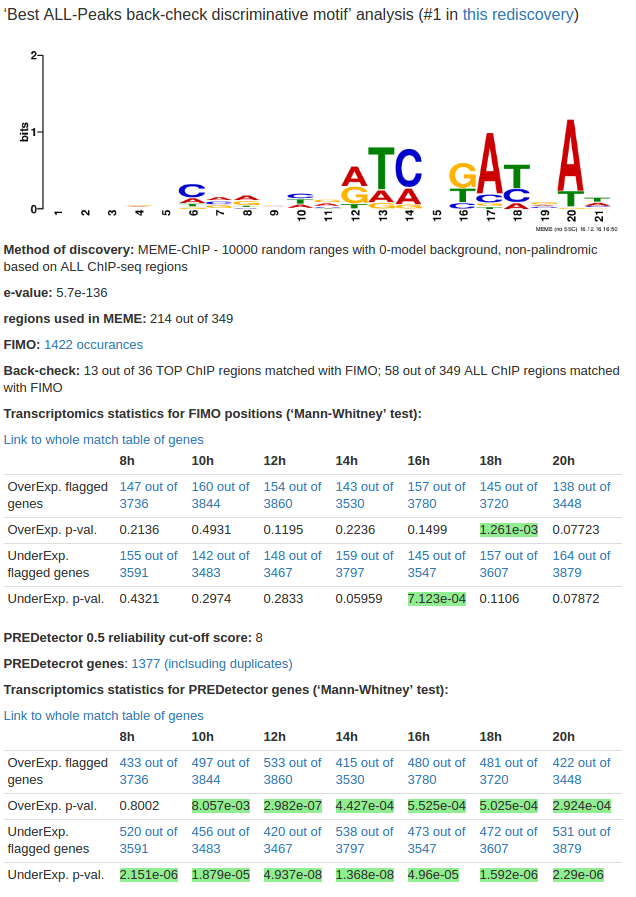
\includegraphics[width=8cm]{stats_motif.png}}
\caption{Statistical analysis output for 'Best ALL-Peaks back-check discriminative motif'. Significant difference in expression between motif/peak related genes and other genes are colored in green}\label{fig:01}
\end{figure}

\begin{figure}[!tpb]%figure1
\centerline{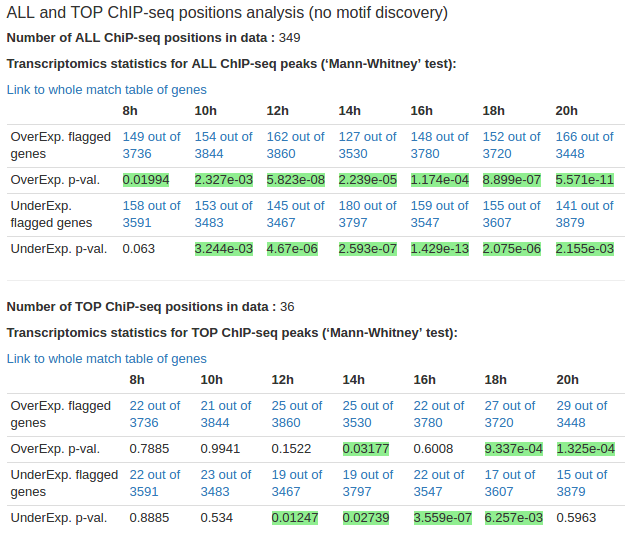
\includegraphics[width=8cm]{chip_seq_stats.png}}
\caption{Statistical analysis output for ALL and TOP ChIP-seq positions analysis (no motif discovery). Significant difference in expression between motif/peak related genes and other genes are colored in green}\label{fig:02}
\end{figure}


\begin{table}[!t]
\processtable{Top 5 Over/Under-expressed gene apperance counts based on all significant lists\label{Tab:01}} {
\begin{tabular}{ l | p{5cm} | c }
\hline
Gene    & Product & Count \\
\cline{1-3}
\multicolumn{3}{c}{Over-Expressed}  \\
\hline
SVEN\_1372 & hypothetical protein & 24   \\
SVEN\_1324 & hypothetical protein    & 24   \\
SVEN\_1278 & Gluconokinase    & 23     \\
SVEN\_1625 & ATP-dependent RNA helicase    & 23    \\
SVEN\_4750 & putative membrane protein & 23 \\
\cline{1-3}
\multicolumn{3}{c}{Under-Expressed} \\
\cline{1-3}
SVEN\_5498 & Transcriptional regulator GntR family & 27  \\
SVEN\_4634 & hypothetical protein & 25  \\
SVEN\_4457 & putative UDP-glucose or GDP-mannose dehydrogenase & 24 \\
SVEN\_2614 & hypothetical protein & 24  \\
SVEN\_0269 & hypothetical protein & 23 \\
\hline
\end{tabular}}{These tables are also available in repository}
\end{table}


\end{methods}



\section{Discussion}

Analyses of four motifs showed that PREDetector gene lists have better significance in statistical test than FIMO positions found from motif (also seen on Figure \ref{fig:01}). That can explained by very simple approach used in FIMO program to identify matches of motif with no relation to genome structure.\\
Analysis of raw ChIP-seq peaks (Figure \ref{fig:02}) showed that genes which are close to these peaks have significant difference of transcription comparing to other genes. So even without motif discovery, results produced based on ChIP-seq peaks only, are one of the best if number of significant times are compared.

\newpage

\section{Conclusion}
The robust procedure and analyses described here confirmed the success of ChIP-seq experiment and produced the lists of ranked genes potentially controlled by WhiH, which will lead to better understanding of its overall regulon in future.


\section*{Acknowledgement}
We are grateful to people working in Bioinformatics department, Biology building, for constant support with overall analysis facilitation and small Linux/R/Rmarkdown tweaks and tricks, which were of great help to get this project done.


\begin{thebibliography}{}
\bibitem[Timothy {\it et~al}., 2013]{Timothy2013} Timothy,Bailey, Pawel,Krajewski, Istvan,Ladunga, Celine,Lefebvre, Qunhua,Li, Tao,Liu, Pedro,Madrigal, Cenny,Taslim, and Jie,Zhang (2013) Practical Guidelines for the Comprehensive Analysis of ChIP-seq Data. {\it PLoS Comput Biol}. 2013 Nov; 9(11): e1003326.

\bibitem[Bush {\it et~al}., 2013]{Bush2013} Bush,M.J., Bibb,M.J., Chandra,G., Findlay,K.C., Buttner,M.J. (2013) Genes required for aerial growth, cell division, and chromosome segregation are
targets of WhiA before sporulation in {\it Streptomyces venezuelae}. {\it mBio}, {\bf 4(5)}: e00684-13. \href{http://dx.doi.org/10.1128/mBio.00684-13}{http://dx.doi.org/10.1128/mBio.00684-13}.

\bibitem[Timothy {\it et~al}., 2009]{MEME} Timothy,L.,Bailey, Mikael,Bod{\'e}n, Fabian,A.,Buske, Martin,Frith, Charles,E.,Grant, Luca,Clementi, Jingyuan,Ren, Wilfred,W.,Li, William,S.,Noble (2009) MEME SUITE: tools for motif discovery and searching. {\it Nucleic Acids Research}, 37:W202-W208.

\bibitem[Pullan {\it et~al}., 2011]{Genome} Pullan,S.T., Chandra,G., Bibb,M.J. and Merrick,M. (2011) Genome-wide analysis of the role of GlnR in Streptomyces venezuelae provides new insights into global nitrogen regulation in actinomycetes. {\it BMC Genomics} {\bf 12}, 175

\bibitem[Hiard {\it et~al}., 2007]{Predetector} Hiard,S, Maree,R, Colson,S, Hoskisson,PA, Titgemeyer,F, van Wezel,GP, Joris,B, Wehenkel,L, Rigali,S. (2007) PREDetector: A new tool to identify regulatory elements in bacterial genomes. {\it Biochem Biophys Res Commun.} 357(4):861-4.


\end{thebibliography}
\end{document}
